\documentclass{article}
\usepackage[utf8]{inputenc}
\usepackage{polyglossia}
\usepackage[table]{xcolor}
\usepackage{graphicx}
\usepackage{multirow}
\usepackage{caption}
\usepackage{enumitem}
\usepackage{tikz}
\usetikzlibrary{shapes,arrows,shadows}
\usepackage{amsmath,bm,times}
\usepackage{systeme}
\usepackage{pdflscape}
\usepackage[american,siunitx]{circuitikz}
\usetikzlibrary{calc,positioning}
\usetikzlibrary{shapes.geometric}
\usepackage{diagbox}
\usepackage{float}
\usepackage{fontspec}
\usepackage{hyperref}
\usepackage{enumitem}

\usepackage{geometry}
\geometry{a4paper,total={170mm,257mm},left=20mm,top=20mm,}

\setsansfont{Arial}

\DeclareCaptionLabelFormat{nospace}{#2#1}
\captionsetup[figure]{labelfont={bf},name={. attēls},labelformat=nospace,labelsep=period}

\renewcommand{\labelenumii}{\theenumii}
\renewcommand{\theenumii}{\theenumi.\arabic{enumii}.}
\renewcommand{\labelenumiii}{\theenumiii}
\renewcommand{\theenumiii}{\theenumii\arabic{enumiii}.}

\newcommand{\mymeter}[2] 
{  % #1 = name , #2 = rotation angle
%\begin{scope}[transform shape,rotate=#2]
\begin{scope}[transform shape]
%\draw[thick] (#1)node(){$\mathbf V$} circle (11pt);
\draw[thick] (#1)node(){$\mathbf #2$} circle (11pt);
%\draw[rotate=45,-latex] (#1)  +(-17pt,0) --+(17pt,0);
\end{scope}
}

\begin{document}

\begin{titlepage}
\begin{center}
\large{Rīgas Tehniskā universitāte \\\vspace{3mm} Elektronikas un telekomunikāciju fakultāte \\\vspace{3mm} Elektronikas pamatu katedra}
\end{center}

\vspace{3cm}

\begin{center}
Datormācība (speckurss)
\end{center}

\begin{center}
10. - 11. nodarbība. LaTeX
\end{center}

\begin{center}
\textbf{Vienkāršu elektrisku shēmu modelēšana}
\end{center}

\vspace{5cm}

\begin{flushright}
Grupas Nr. REBM01
 \end{flushright}

 \begin{flushright}
Stanislavs Tarasovs
 \end{flushright}
 
 \begin{flushright}
Studenta apliecības Nr. 191REB142
 \end{flushright}

\vfill
\begin{center}
\scshape{Rīga,2020}
\end{center}
\end{titlepage}

\vspace{0.25cm}
    
\textbf{Darba mērķi}
\begin{itemize}
    \item Iemācīties veidot dokumentus, izmantojot LaTeX
\end{itemize}

\section{Teorētiska daļa}
    \begin{center}
\begin{circuitikz}[american]

\draw (0,2) to[short,-] (3,2);
\draw (0,-2) to[short,-] (3,-2);
\draw (3,-2) to[short,*-*] (3,-2);
\draw (3,0) to[short,*-*] (3,0);
\draw (3,-2) to[short,-] (5,-2);
\draw (3,0) to[short,-] (5,0);

\draw (0,2) to[voltage source,l_=$U_\text{in}$] (0,-2);
\draw (3,2) to[generic,l=$R_1$] (3,0);
\draw (3,0) to[generic,l=$R_2$] (3,-2);

\node (A) at (5,-0.25) {};
\node (B) at (5,-1.75) {};
\draw[thick,color=blue,->] (A) -- (B) node[midway,sloped,left,rotate=90] {$U_\text{out}$};
\node (C) at (0.65,0.5) {};
\node (D) at (0.65,-0.5) {};
\draw[thick,color=blue,->] (C) -- (D) node[midway,sloped,right,rotate=90] {$U_\text{in}$};

\end{circuitikz}
\captionof{figure}{Sprieguma dalītāja shēma} \label{figure:2lw1s}
\end{center}
    Vērtības no 9. nodarbības(izmantojot studenta apliecības numuru):\\$U_\text{in}$ = 14.2 V\\$R_1$ = 5 $\Omega$\\$R_2$ = 3 $\Omega$\\\\
    Izejas sprieguma formula: \begin{equation}U_\text{out} = \frac{U_\text{in}\cdot R_2}{R_1 + R_2} = \frac{14.2\cdot 3}{8} = 5.325 V,\label{eq1}\end{equation}kur\\$U_\text{in}$ - ieejas spriegums,\\$U_\text{out}$ - izejas spriegums,\\$R_1$ - pirma rezistora vērtība,\\$R_2$ - otra rezistora vērtība.\\\\
    
\newpage
\section{Eksperimentālā daļa}
    \subsection{Shēmas zīmēšana (GSchem)}
        Izmantojot GSchem, es uzzīmēju sprieguma dalītāja shēmu. GSchem es palaidu ar konsoles palīdzību, izmantojot komandu "gschem". Pēc tam atvērās Gschem logs:\\
        \begin{figure}[H]\centering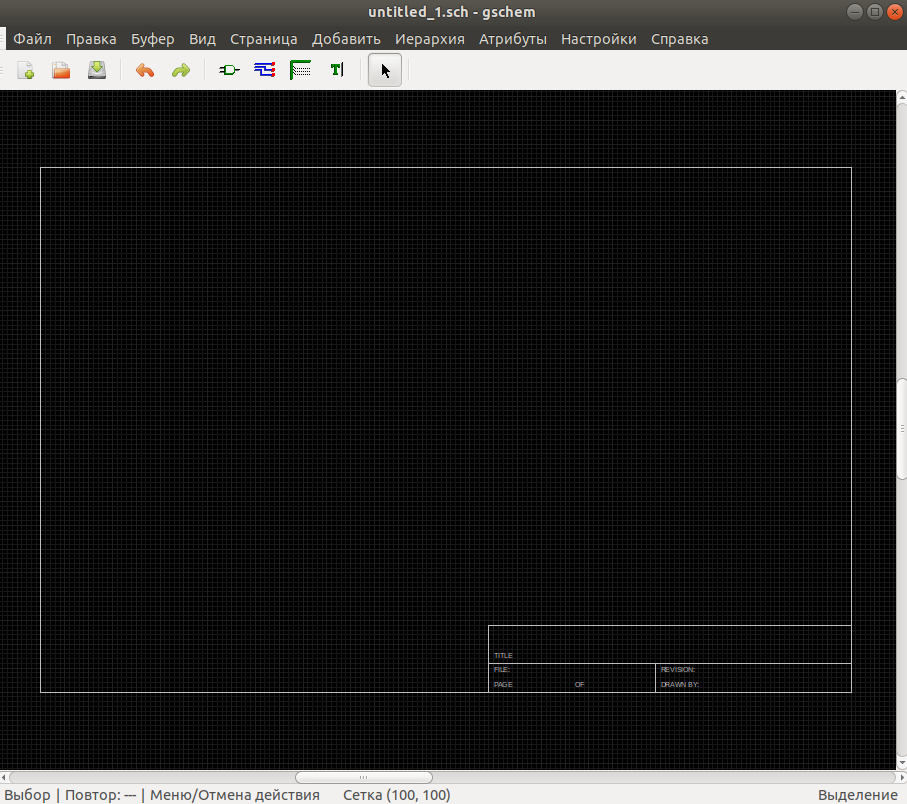
\includegraphics[width=0.60\textwidth]{pictures/gschem1.PNG}\caption{GSchem logs}\label{picture:10lw1p}\end{figure}
        
        Ar "Add component" palīdzību, es ievietoju komponentes. Piemēram, kā es ievietoju "voltage source" :
        
        \begin{figure}[H]\centering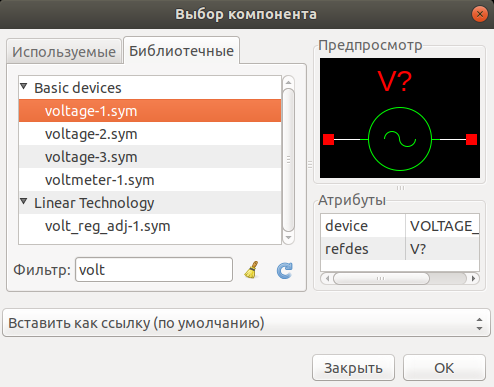
\includegraphics[width=0.60\textwidth]{pictures/gschem2.PNG}\caption{GSchem "Add component" logs}\label{picture:10lw2p}\end{figure}
        \newpage
        
        Pēc tam savienoju visus elementus ar vadiem, ievietoju zemi un katram komponentam norādīju vērtības, pievienojot "Value" vērtību katram elementam.
        
        \begin{figure}[H]\centering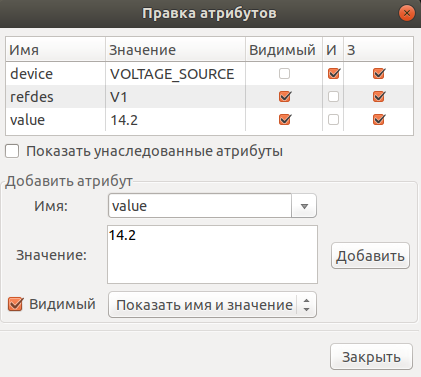
\includegraphics[width=0.60\textwidth]{pictures/gschem4.PNG}\caption{GSchem "Value" vērtības pievienošana}\label{picture:10lw3p}\end{figure}
        
        \begin{figure}[H]\centering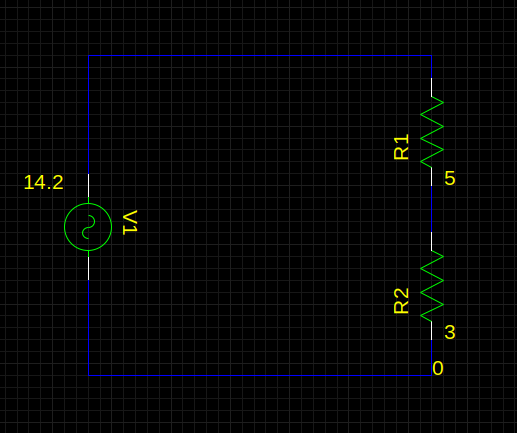
\includegraphics[width=0.60\textwidth]{pictures/gschem3.PNG}\caption{GSchem "Voltage\_divider" shēma}\label{picture:10lw4p}\end{figure}
    
    \newpage
    \subsection{Elementu-mezglu faila izveidošana (gnetlist)}
        Šīs fails mums ir vajadzīgs, lai veiktu shēmas simulāciju. Fails saturēs elementu vērtības un mezglus pie kuriem šie elementi ir savienoti. Lai izveidotu šo failu es izmantoju gnetlist komandu :
        
        gnetlist -g spice -o voltage\_divider.net voltage\_divider.sch,\\
        kur\\
        voltage\_divider.net - fails ar elementu-mezglu sarakstu\\
        voltage\_divider.sch - shēmas fails\\
        
         Ja shēmā viss ir izdarīts pareizi, tad pēc "Loading schematic" komandas izveidosies fails voltage\_divider.net:
         
         \begin{figure}[H]\centering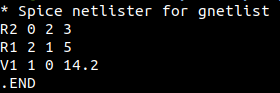
\includegraphics[width=0.60\textwidth]{pictures/gnetlist.PNG}\caption{Pēc gnetlist jauns "voltage\_divider.net" fails}\label{picture:10lw5p}\end{figure}
         
    \subsection{Shēmas simulācija}
        Izmantojot NGSpice, es varēju veikt shēmas simulāciju.
        Lai veiktu simulāciju, pirmkārt, vajag konsolē uzrakstīt "ngspice", lai to palaist:
        
         \begin{figure}[H]\centering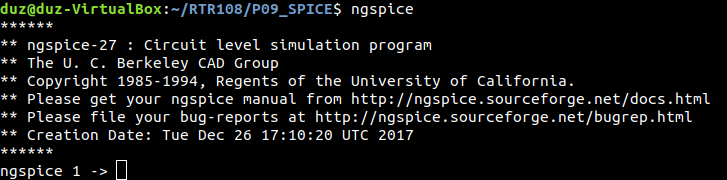
\includegraphics[width=0.60\textwidth]{pictures/ngspice1.PNG}\caption{NGSpice konsolē}\label{picture:10lw6p}\end{figure}
        
        Otrkārt, vajag uzrakstīt "source" komandu, kura norāda failu, kuram tiks veikta simulācija :
        
        \begin{figure}[H]\centering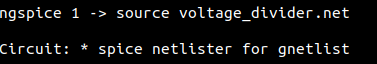
\includegraphics[width=0.60\textwidth]{pictures/ngspice2.PNG}\caption{NGSpice source komanda}\label{picture:10lw7p}\end{figure}
        
        Pēc tam izmantosim komandu "tran solis beigas sākums", kura veiks transient simulāciju laika posmā. Pēc simulācijas veikšanas parādīsies simulācijas rezultāti:
        
        \begin{figure}[H]\centering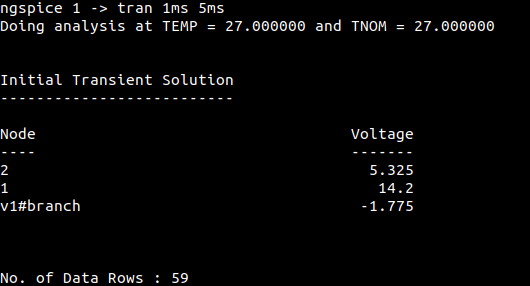
\includegraphics[width=0.60\textwidth]{pictures/ngspice3.PNG}\caption{NGSpice tran simulācija}\label{picture:10lw8p}\end{figure}
        
        Pēc simulācijas veikšanas, vajag uzzīmēt un izvadīt simulācijas grafikus. Izmantojam komandu " plot "mezgls" ", kura izvada grafiku un "hardcopy faila nosaukums "mezgls" ", kura izvadīs grafiku failā:
        
        \begin{figure}[H]\centering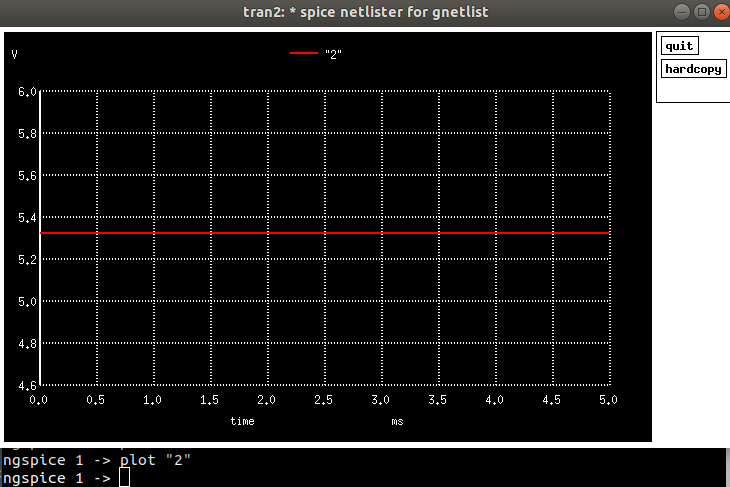
\includegraphics[width=0.60\textwidth]{pictures/ngspice4.PNG}\caption{NGSpice plot komanda}\label{picture:10lw9p}\end{figure}
        
        \begin{figure}[H]\centering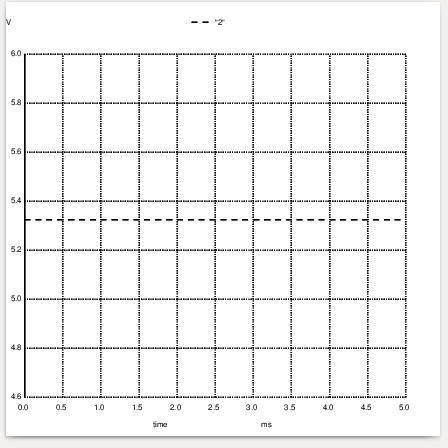
\includegraphics[width=0.45\textwidth]{pictures/ngspice5.PNG}\caption{NGSpice hardcopy komanda}\label{picture:10lw10p}\end{figure}
    
    \newpage
    \section{Rezultātu apkopojums un secinājumi}
        \begin{center}
    \begin{tabular}{|c|c|}
    \hline
    &$U_{out}, \mathrm{V}$\\
    \hline
    Teorētiskie aprēķini&5.325\\
    \hline
    Shēmas simulācija&5.325\\
    \hline
    \end{tabular}
\end{center}
        Ir redzams, ka teorētikie un simulācijas rezultāti sakrīt, tāpēc es varu secināt, ka viss bija izdarīts pareizi. Secinājumā, visi darba mērķi bija izpildīti.
\end{document}